\section{Стандартная ошибка среднего}

Предположим, что $x$ -- вещественная случайная величина с распределением вероятностей $F$. Обозначим математическое ожидание и дисперсию $F$ символами $\mu_F$ и $\sigma^2_F$ соответственно,
\begin{equation}
    \mu_F=E_F(x),\qquad \sigma^2_F=var_F(x)=E_F[(x-\mu_F)^2].
\end{equation}
В главе 3 эти величины назывались $\mu_x$ и $\sigma^2_x$. Здесь мы подчеркиваем зависимость от $F$. Альтернативное обозначение $var_F (x)$ для дисперсии, иногда сокращенное до $var (x)$, означает то же самое, что и $\sigma^2_F$. В дальнейшем мы иногда будем писать
\begin{equation}
    x\sim(\mu_F,\sigma^2_F)
\end{equation}
чтобы кратко обозначить математическоу ожидание и дисперсию $x$.

Теперь пусть $(x_1,\cdots, x_n)$ будет случайной выборкой размера $n$ из распределения $F$. Среднее значение выборки $\bar x = \sum_{i=1}^n x_i / n$ имеет математическое ожидание $\mu_F$ и дисперсию $\sigma^2_F/n$, 
\begin{equation}
    \bar x\sim(\mu_F,\sigma^2_F/n).
\end{equation}
Другими словами, математическоу ожидание $\bar x$ такое же, как ожидание одного $x$, но дисперсия $\bar x$ равна $1 / n$ дисперсии $x$. Это причина использования средних значений: чем больше $n$, тем меньше $var (\bar x)$, поэтому большее $n$ означает лучшую оценку $\mu_F$·

Стандартная ошибка среднего $\bar x$, записанная как $se_F (\bar x)$ или $se (\bar x)$, является квадратным корнем из дисперсии $\bar x$, 
\begin{equation}
    se_F (\bar x) = [var_F(\bar x)]^{1/2} = \sigma_F/\sqrt{n}.
\end{equation}
Стандартная ошибка -- это общий термин для стандартного отклонения сводной статистики. Это наиболее распространенный способ индикации статистической точности. Грубо говоря, мы ожидаем, что $|\bar x-\mu_F|$ будет меньше одной стандартной ошибки примерно в 68\% случаев и меньше двух стандартных ошибок примерно в 95\% случаев. 

Эти проценты основаны на центральной предельной теореме. При довольно общих условиях на $F$ распределение $\bar x$ будет приблизительно нормальным при увеличении $n$, что мы можем записать как 
\begin{equation}
    \bar x\sim N(\mu_F,\sigma^2_F/n).
\end{equation}
Математическое ожидание $\mu_F$ и дисперсия $\sigma^2_F/n$ в (5.5) точны, только нормальность является приблизительной. Используя (5.5), таблица нормального распределения дает 
\begin{equation}
    Prob\{|\bar x - \mu_F|<\frac{\sigma_F}{\sqrt{n}}\}=0.683\qquad Prob\{|\bar x - \mu_F|<\frac{2\sigma_F}{\sqrt{n}}\}=0.954,
\end{equation}
как показано на Рисунке 5.1. Одно из преимуществ бутстрепа заключается в том, что не нужно полностью полагаться на центральную предельную теорему.
\newline

\noindent
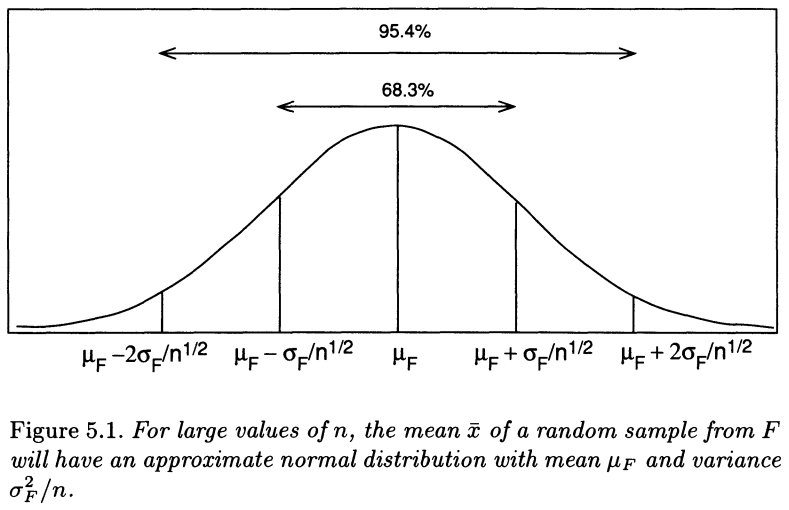
\includegraphics[width=\linewidth]{4/f51.png}
\newline
Простой пример показывает ограничения аппроксимации центральной предельной теоремы. Предположим, что $F$ -- это распределение, которое ставит вероятность только для двух исходов, 0 или 1, скажем 
\begin{equation}
    Prob\{x=1\}=p\qquad Prob\{x=0\}=1-p.
\end{equation}
Здесь $p$ -- параметр $F$, часто называемый вероятностью успеха, имеющий значение от 0 до 1. Случайная выборка $F \rightarrow (x_1, x_2,\cdots, x_n)$ может рассматриваться как $n$ независимых подбрасываний монеты с вероятностью успеха (или «орла», или $x = 1$) равной $p$. Тогда сумма $s = \sum_{i=1}^nx_i$ -- количество успехов в $n$ независимых бросках монеты; $s$ имеет биномиальное распределение (3.3), 
\begin{equation}
    s\sim Bi(n,p).
\end{equation}
Среднее значение $\bar x = s / n$ равно $\hat p$ в плагин оценке $p$ Распределение (5.7) имеет $\mu_F=p$, $\sigma^2_F = p (1- p)$, поэтому (5.3) дает 
\begin{equation}
    \hat p\sim (p,p(1-p)/n)
\end{equation}

для среднего и дисперсии $\hat p$ Другими словами, $\hat p$ -- это несмещенная оценка $p$, $E (\hat p) = p$, со стандартной ошибкой 
\begin{equation}
    se(\hat p)=\left[\frac{p(1-p)}{n}\right]^{1/2}.
\end{equation}
\newline

\noindent
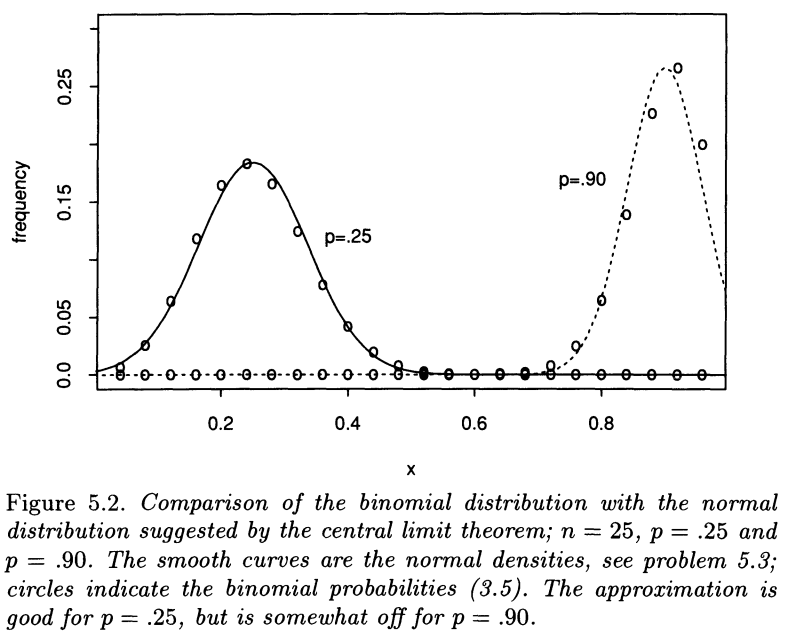
\includegraphics[width=\linewidth]{4/f52.png}
\newline
На рис. 5.2 показана центральная предельная теорема, работающая для биномиального распределения при $n = 25$, $p = 0.25$ и $p = 0.90$. Центральная предельная теорема дает хорошее приближение к биномиальному распределению для $n = 25$, $p = 0.25$, но несколько хуже для $n = 25$, $p = 0.9$. 